\documentclass[10pt,twocolumn,letterpaper]{article}
            
\usepackage[pagenumbers]{iccv}

\newcommand{\red}[1]{{\color{red}#1}}
\newcommand{\todo}[1]{{\color{red}#1}}
\newcommand{\TODO}[1]{\textbf{\color{red}[TODO: #1]}}

\definecolor{iccvblue}{rgb}{0.21,0.49,0.74}
\usepackage[pagebackref,breaklinks,colorlinks,allcolors=iccvblue]{hyperref}
\usepackage{svg}
\usepackage{makecell}
\usepackage{graphicx}
\usepackage{array}
   \usepackage{booktabs} 
   \usepackage{multirow} 

\def\paperID{10}
\def\confName{ICCV}
\def\confYear{2025}

\title{用于实时四旋翼控制的高效自监督神经解析视觉伺服}

\author{
Sebastian Mocanu\textsuperscript{1} \quad
Sebastian-Ion Nae\textsuperscript{1}\thanks{These authors contributed equally to this work.} \quad
Mihai-Eugen Barbu\textsuperscript{1}\footnotemark[1] \quad
Marius Leordeanu\textsuperscript{1, 2, 3} \\
\textsuperscript{1}National University of Science and Technology POLITEHNICA Bucharest, Romania \\
\textsuperscript{2}Institute of Mathematics "Simion Stoilow" of the Romanian Academy, Romania \\
\textsuperscript{3}NORCE Norwegian Research Center, Norway \\
{\footnotesize\ttfamily\ \{sebastian.mocanu, sebastian\_ion.nae.stud.fils, mihai\_eugen.barbu.stud.acs\}@upb.ro, leordeanu@gmail.com} 
}

\begin{document}
\maketitle

\begin{abstract}
本文提出一种面向视觉四旋翼控制的自监督神经解析模型。该模型在计算上较为高效，由一个仅含 1.7M 参数的学生卷积网络从一个解析式教师模型中自动学习，而教师模型则是改进后的基于图像的视觉伺服（IBVS）控制器。我们通过降低经典视觉伺服方程的复杂度并增强图像特征检测的稳定性，解决了 IBVS 系统中的数值不稳定问题。借助知识蒸馏，学生模型的推理速度比教师 IBVS 管线快 $11\times$，同时在控制精度上保持相近水平，而计算和存储开销则显著降低。

这种仅依赖视觉的自监督神经解析控制方式，无需显式几何模型或 fiducial marker，即可实现四旋翼的姿态调整与运动控制。所提方法结合了仿真到现实的迁移学习，并在无 GPS 的室内环境中、基于小型无人机平台进行了验证。本文的主要贡献包括：(1) 提出一种能够解决经典方法中固有数值不稳定问题的解析式 IBVS 教师模型；(2) 构建由 YOLOv11 与基于 U-Net 的掩码分裂器组成的两阶段分割流程，用于稳健地将车辆前后区域分开并正确估计目标朝向；(3) 设计一种高效的双路径知识蒸馏系统，将教师模型的几何视觉伺服能力迁移到紧凑型学生神经网络中，使其在优于教师模型的同时，适合实时机载部署。
\end{abstract}

\section{引言}
\label{sec:intro}
四旋翼无人机的应用已经从遥控飞行器扩展到用于航拍、测绘和配送的自主系统，通常依赖 GPS、IMU 以及 9 自由度传感器融合 \cite{arreola2018improvement}。虽然这些传感器在室外环境中效果较好，但在室内环境下会因信号干扰、多路径效应和标定误差而性能下降 \cite{tang2024control, rebbapragada2024c2fdrone}。基于视觉的传感器成本更低，并且能够通过直接感知环境和即时视觉反馈来弥补这些不足，从而在无 GPS 环境中实现实时特征提取和空间感知。

需要四旋翼与目标对象之间保持空间协调的任务，例如自动仓库巡检系统 \cite{wawrla2019applications} 和动态影视拍摄 \cite{nageli2017real}，都需要鲁棒的视觉伺服方法。在仓储维护场景中，无人机必须在补偿环境扰动的同时，与基础设施部件保持特定距离 \cite{kouris2018learning} 和观看角度 \cite{wawrla2019applications}。类似地，在影视应用中，随着目标沿复杂轨迹运动，系统需要持续调整位姿以维持期望构图 \cite{galvane2017automated}。

视觉伺服使用闭环反馈，将期望图像特征与当前测量值进行比较，并把特征坐标和几何属性直接作为控制输入，而无需显式进行三维位姿重建 \cite{hutchinson1996tutorial, guenard2008practical}。然而，经典基于图像的视觉伺服（IBVS）方法常常会因为交互矩阵中的奇异性以及大范围相机运动中的病态条件而产生数值不稳定 \cite{corke1996visual}。在目标跟踪和位姿对齐任务中，通常会使用 ArUco \cite{kalaitzakis2021fiducial, mraz2020using, cruz2024performance} 或 AprilTag \cite{olson2011apriltag, zhang2017autonomous, banik2025integrating} 等 fiducial marker，这些标记提供了易于检测且具有预定义几何特征的目标，但这类方法仍然面临计算挑战以及对标记的依赖，从而限制了其在动态、无结构室内环境中的部署。

本文提出一种高效的无标记方法。该方法使用一个自监督的解析式 IBVS 教师模型，通过对经典方程进行简化并增强图像特征检测，来解决数值不稳定问题；同时结合一个轻量级学生神经网络，以获得更优的实时性能。所提自监督教师方法采用两阶段神经网络流程：第一阶段使用 YOLO \cite{redmon2016you, riftiarrasyid2024suitability, yang2025comparative} 实例分割网络完成目标检测；第二阶段将生成的掩码一分为二，以估计玩具车目标的朝向（前后分割），从而在不依赖 fiducial marker 的情况下实现精确的无人机定位。该知识蒸馏框架把改进 IBVS 教师的解析稳定性迁移到一个更高效、成本更低的学生网络中，同时还获得了更好的控制性能。系统验证采用渐进式流程，先进行仿真训练，再引入真实世界数据进行微调。

实验装置只需要一台普通笔记本电脑和一条与四旋翼平台相连的无线通信链路，硬件需求极低，这说明该方法在室内自主运行方面具有现实可行性，同时也面向未来的边缘部署应用。

\section{基于视觉的伺服}
\label{sec:related_work}
视觉伺服是移动机器人中一种基础的控制范式，它利用基于摄像头的反馈进行运动引导。经典方法通常分为基于位置的视觉伺服（PBVS）和基于图像的视觉伺服（IBVS）两类。PBVS 通过图像特征重建三维位姿，并在笛卡尔空间中进行控制 \cite{qin2023perception, sun2025towards}；而 IBVS 则直接把图像特征作为反馈信号，从而规避位姿估计的不确定性 \cite{corke1996visual, yang2020autonomous, lee2012adaptive}。对于实时机器人应用，由于其计算效率高且鲁棒性较好，IBVS 更常被采用 \cite{yang2024high, kumar2024tracking}。

IBVS 控制律可表示为：

\begin{equation}
\mathbf{v} = -\lambda \mathbf{L}_s^+ (\mathbf{s} - \mathbf{s}^*)
\end{equation}

其中，$\mathbf{v} = [v_x, v_y, v_z, \omega_x, \omega_y, \omega_z]^T$ 表示摄像机速度螺旋量（线速度和角速度），$\lambda$ 为控制增益，$\mathbf{s}$ 为当前图像特征，$\mathbf{s}^*$ 为期望特征。

交互矩阵 $\mathbf{L}_s$（图像雅可比）描述了特征运动与相机运动之间的关系：

\begin{equation}
\dot{\mathbf{s}} = \mathbf{L}_s \mathbf{v}
\end{equation}

对于像素坐标为 $(u,v)$、深度为 $Z$ 的每个点，其交互矩阵为：

\begin{equation}
\label{eq:ibvs-full}
\mathbf{L}_s = \begin{pmatrix}
-\frac{f}{Z} & 0 & \frac{\bar{u}}{Z} & \frac{\bar{u} \bar{v}}{f} & -\frac{f^2 + \bar{u}^2}{f} & \bar{v} \\
0 & -\frac{f}{Z} & \frac{\bar{v}}{Z} & \frac{f^2 + \bar{v}^2}{f} & -\frac{\bar{u} \bar{v}}{f} & -\bar{u}
\end{pmatrix}
\end{equation}

其中，$\bar{u} = u - u_0$ 和 $\bar{v} = v - v_0$ 是相对于主点的像素坐标，$f$ 是以像素为单位表示的焦距。

伪逆 $\mathbf{L}_s^+$ 可表示为：

\begin{equation}
\mathbf{L}_s^+ = (\mathbf{L}_s^T \mathbf{L}_s)^{-1} \mathbf{L}_s^T
\end{equation}

特征检测是 IBVS 实现中的关键环节。由于可靠性高且实现简单，基于标记点的方法长期占据主流。Inria 已在 Parrot Bebop 2 平台上演示了用于运动目标任务的 ArUco 标记跟踪 \cite{Marchand05b}，也演示了基于 PID 的运动目标跟踪 \cite{teuliere2011chasing}。类似的基于标记点系统也已应用于自动降落和表面检测任务 \cite{keipour2022visual, drones8110605}，并在真实场景中证明了其有效性。

然而，基于标记点的方法在实际应用中存在局限，例如对环境条件变化敏感，如光照变化、部分遮挡和标记退化等。此外，标记的安装和维护要求也限制了其在动态或难以进入的环境中的适用性 \cite{liang2020moving}。

近年来，深度学习的发展引入了其他特征检测方法。神经网络作为关键点检测器已被用于特定目标跟踪，例如 \cite{sepahvand2025deep} 中使用 CNN 在不同光照和遮挡条件下检测矩形目标的关键点。其他工作则关注在激烈机动过程中进行边界框检测和目标中心跟踪 \cite{10140151}。
YOLO 系列模型已被广泛应用于机器人领域 \cite{li2023design, zhang2024vision}，包括实例分割 \cite{mohamed2021insta, tang2024visual}、目标检测 \cite{drones8110605} 和图像分类 \cite{zhao2024real}，这说明深度学习方法在视觉伺服特征提取中的通用性 \cite{pathre2024imagine2servo}。

近期方法开始将神经网络与视觉伺服算法结合，以增强机器人控制能力。Liu 等人 \cite{liu2019image} 提出了一种用于机械臂操作的双流网络，可直接输出速度命令，在无需显式视觉伺服计算的情况下实现期望位姿。知识蒸馏技术在轻量化伺服网络中也显示出潜力，例如 \cite{drones8110605} 中，学生网络学习了树枝操作中的最佳抓取点识别。

本文在这些研究基础上继续推进，将 YOLO 分割网络与 IBVS 算法结合并进行知识蒸馏，从而在保持计算效率的同时消除对 fiducial marker 的依赖。所提出的轻量级网络能够直接从单帧相机图像生成速度命令。此外，本文还通过持续学习来缩小仿真到现实之间的差距，先在仿真环境中训练，再用真实世界数据进行微调，以保证其在不同部署环境中的鲁棒性。

\section{Our Approach}
\label{sec:proposed_method}
\begin{figure*}[t]
    \centering
    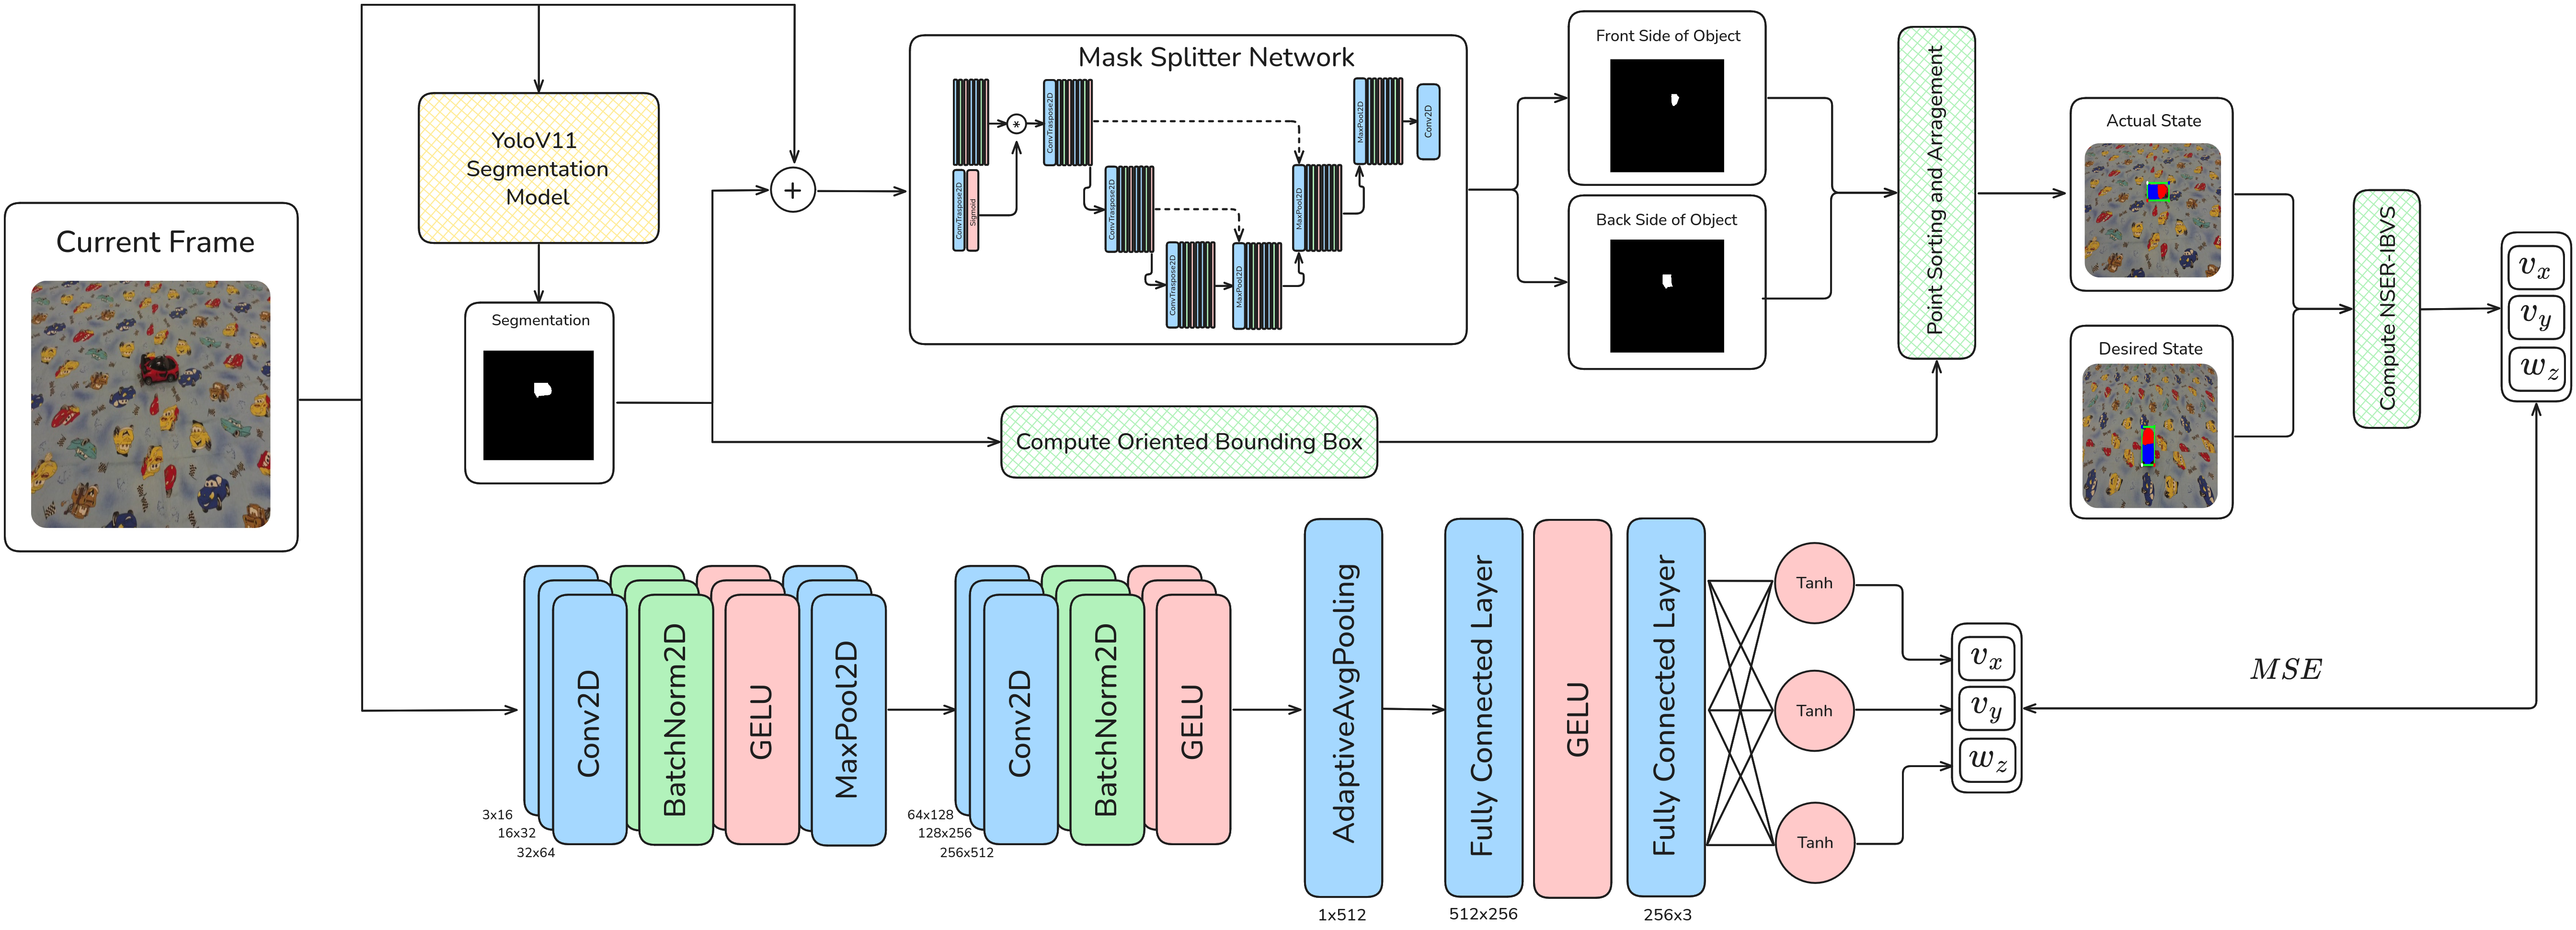
\includegraphics[width=\textwidth]{teacher-student-math.png}
    \caption{Overview of the proposed Teacher-Student Self-supervised Neuro-Analytic model. Top row illustrates the NSER-IBVS (analytical) Teacher path, which uses YOLO for object segmentation and a mask splitter network to estimate object orientation relative to the drone camera. The bottom one represents the Student path, which learns by minimizing the MSE cost between its output drone commands ($\nu_x$, $\nu_y$, $\omega_z$) and the Teacher's output.}
    \label{fig:teacher-student-math}
\end{figure*}

Our method consists of a teacher-student framework for vision-based quadrotor control, both teacher and student are tested in a digital-twin of the real-world environment. 

The teacher employs a two-stage neural network processing system that is combined with an image-based visual servoing algorithm. In the first stage, a small YOLOv11 Nano (2.84M parameters) instance segmentation network is used. This network is initially trained on synthetic data from the digital-twin and subsequently fine-tuned using real images. This stage has two main objectives: to compute an oriented bounding box (OBB) of the car and to provide its mask to the second stage of our system, as the OBB alone is insufficient for accurate pose inference. The second stage is a specialist neural network trained to split the YOLO masks in half, generating masks that represent the front and back regions of the target vehicle. Knowing the position of these front and back masks and having the OBB, we can rearrange the keypoints to generate four ordered points (two per region) that serve as stable visual features for IBVS. The image Jacobian and control velocities are computed using these features to minimize the error and achieve the desired relative state. The desired orientation keypoints are established by capturing the target pose at the beginning, applying segmentation, and extracting the corresponding feature points. Then we preprocess these  keypoints for stability enhancement, detailed in Section \ref{sec:ibvs_implem}. Our method then rectifies its pose with respect to the desired reference pose.

This framework constitutes the teacher model, which is distilled into a compact convolutional neural network trained via regression to output quadrotor control velocities from camera input RGB images detailed in Section \ref{sec:know_dist}.


\begin{figure*}[t]
    \centering
    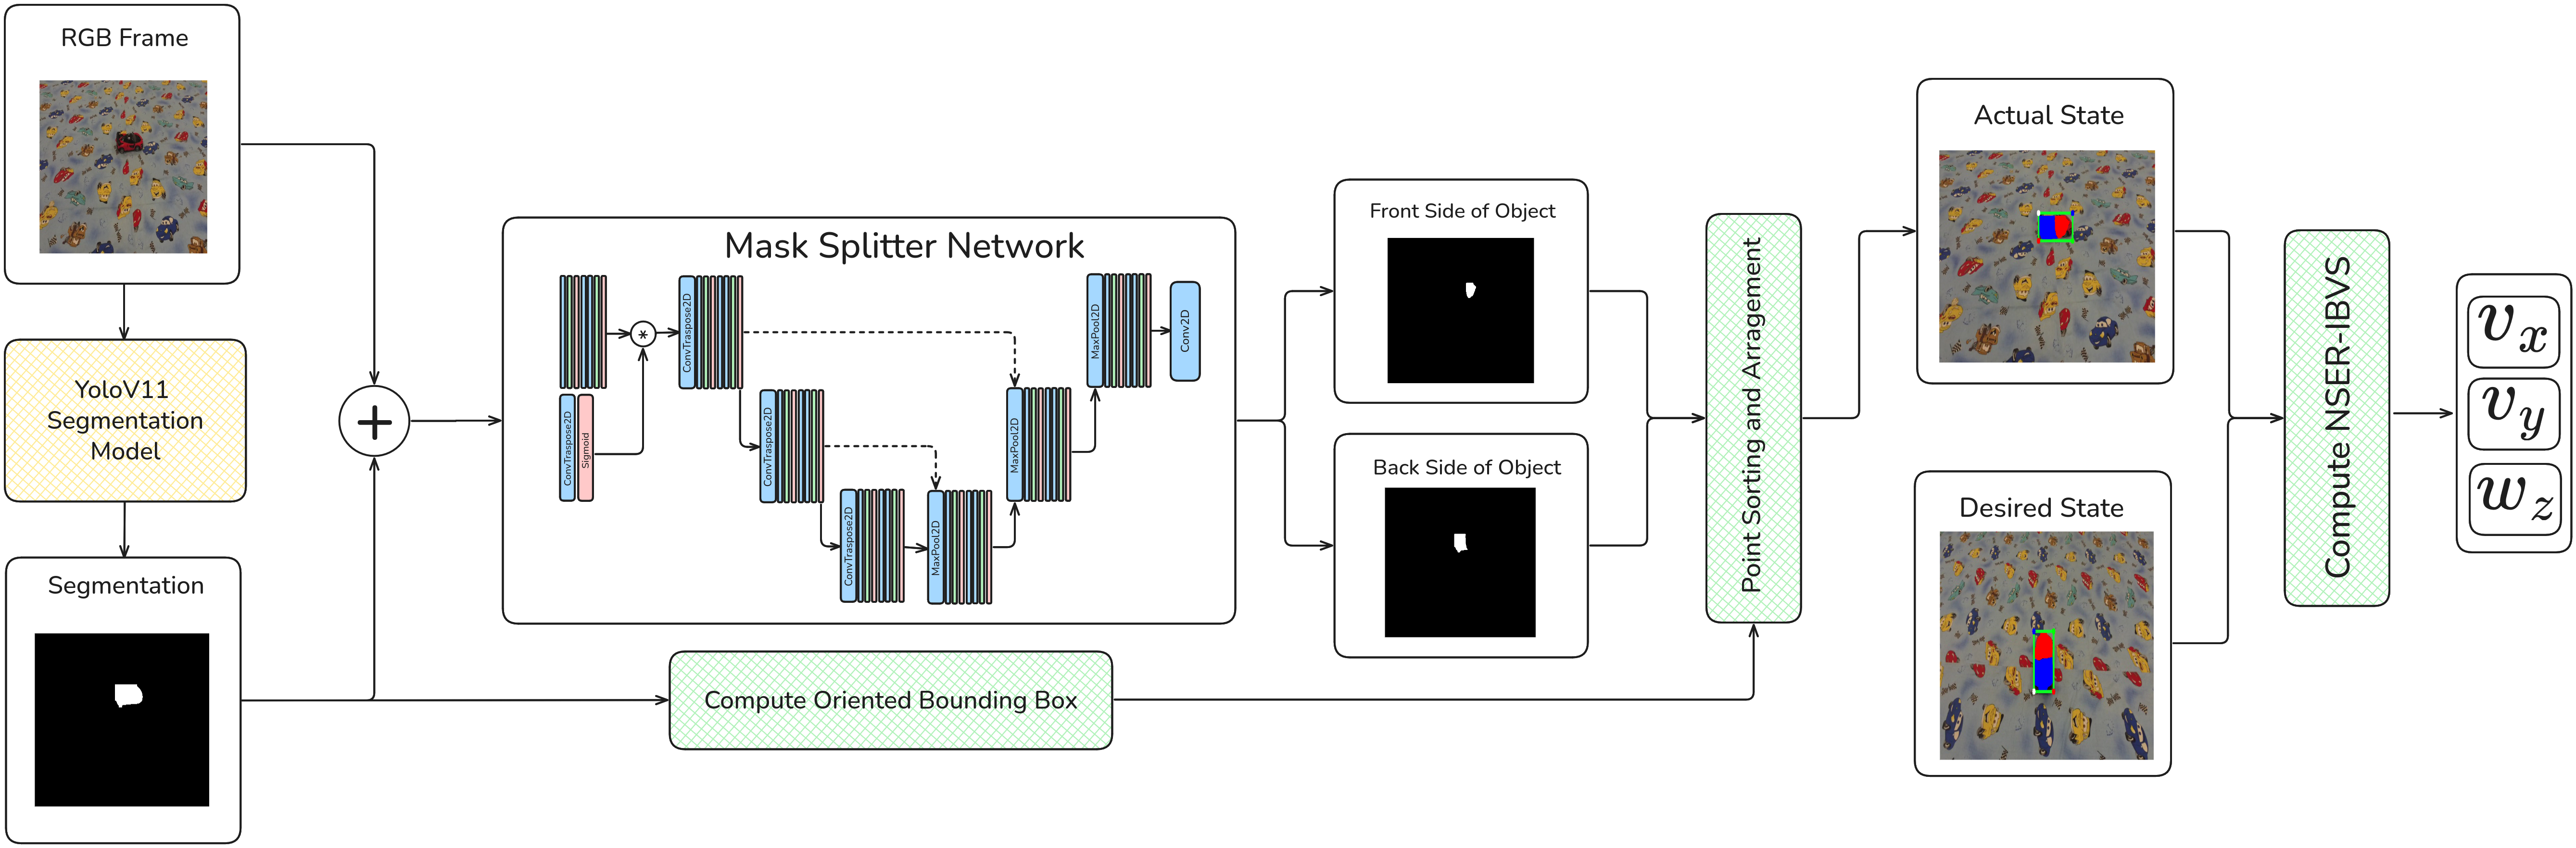
\includegraphics[width=\textwidth]{NSER-IBVS.png}
    \caption{Overview of the proposed Numerically Stable, Efficient, Reduced Image Based Visual Servoing (NSER-IBVS) architecture. The pipeline takes an RGB frame, generates segmentation, and feeds them as input to the Mask Splitter Network. From the original segmentation, bounding box coordinates are determined and used together with the divided front and back masks to rearrange coordinates positions. These coordinates serve as visual features for the analytical model to compute the velocity commands ($\nu_x$, $\nu_y$, $\omega_z$).}
    \label{fig:nser-ibvs}
\end{figure*}

\subsection{Numerically Stable Efficient Reduced IBVS}
\label{sec:ibvs_implem}

The proposed method begins by training a YOLOv11 Nano instance segmentation model using simulation-generated data, forming the foundation of a two-stage segmentation pipeline. The first stage segments the entire vehicle, while a secondary network splits the segmented region into anterior and posterior components, as illustrated in Figure \ref{fig:nser-ibvs}. While effective for segmentation, the first stage generates bounding boxes that may include parts not belonging to the object. To address this issue, we compute a bounding box around the segmented object mask. This produces an unstable point ordering at inference time, introducing inconsistencies for the analytical IBVS algorithm. By determining the positions of the frontal and rear masks, we can rearrange these points to create an oriented bounding box that better represents the car pose and provides more stable feature points, as shown in Figure \ref{fig:bb-vs-obb-yolo-seg}.

\begin{figure}[!ht]
    \centering
    \begin{minipage}[b]{0.31\linewidth}
        \centering
        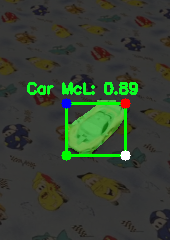
\includegraphics[width=\linewidth]{car-seg-simple.png}
    \end{minipage}
    \hfill
    \begin{minipage}[b]{0.31\linewidth}
        \centering
        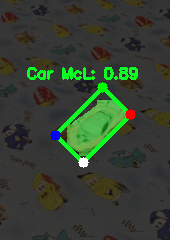
\includegraphics[width=\linewidth]{car-seg-semi-oriented.png}
    \end{minipage}
    \hfill
    \begin{minipage}[b]{0.31\linewidth}
        \centering
        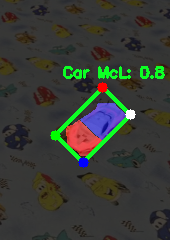
\includegraphics[width=\linewidth]{car-seg-mask-splitter.png}
    \end{minipage}
    \caption{Comparison of different bounding box approaches derived from segmentation results: (left) regular bounding box including parts that do not belong to the object, (middle) oriented bounding box that may vary in orientation between frames, and (right) oriented bounding box using a mask-splitting network to separate anterior and posterior vehicle components for improved ordering stability.}
    \label{fig:bb-vs-obb-yolo-seg}
\end{figure}


The mask splitting network employs a U-Net \cite{ronneberger2015unetconvolutionalnetworksbiomedical} architecture with attention mechanisms \cite{oktay2018attentionunetlearninglook}, accepting a 4-channel input tensor that comprises the original RGB image and the binary vehicle mask from YOLOv11. The encoder-decoder structure features skip connections and progressively downsamples through three stages with channel dimensions of 32, 64, 128, and 256. An attention mechanism applied to the mask channel generates spatial weights that modulate image features to focus on vehicle regions. The decoder reconstructs spatial resolution through transposed convolutions, producing a 2-channel output that represents anterior and posterior segmentation masks. The network contains approximately 1.94M parameters and incorporates dropout regularization in deeper layers preventing overfit.

The splitter loss function partitions a binary segmentation mask into complementary front and back regions by reconstructing the original input mask. Multiple constraints enforce proper partitioning: individual binary cross-entropy losses ensure that each predicted mask matches its ground truth target, a partition constraint penalizes deviations when the sum of both predicted masks differs from the original mask, and overlap penalties discourage simultaneous occupancy of the same pixels. The coverage loss ensures accurate reconstruction by penalizing both excess predictions beyond the original mask and the missed areas within it. Loss weights are dynamically scheduled during training, emphasizing individual mask accuracy, then gradually shifting toward stronger partition and overlap constraints.

The resulting segmentation masks are processed to compute an oriented bounding box by fitting the minimum enclosing rectangle to the object boundary. The four corner coordinates of this bounding box serve as visual features of the IBVS framework. To ensure keypoint stability and consistent ordering, we employ a preprocessing algorithm that assigns points to anterior or posterior regions based on their proximity to the respective mask centroids. The points are subsequently ordered clockwise to maintain temporal consistency across frames, thereby preventing feature correspondence ambiguity that could destabilize the IBVS control loop.

Control velocity computation is achieved by comparing current keypoint coordinates with reference features obtained from a desired pose configuration. Due to the underactuated nature of the quadrotor platform, we use an efficient approach to compute only the necessary velocity components from the classical IBVS controller by eliminating the angular velocity components $\omega_x$ and $\omega_y$ and the linear velocity $\nu_z$. Furthermore, since our controller operates exclusively at fixed altitude, we also remove the linear velocity component $v_z$. 

Starting from Equation \ref{eq:ibvs-full}, the reduced interaction matrix takes the form:
\begin{equation}
\label{eq:numerical-stable-efficient-reduced-ibvs}
\begin{pmatrix}
\dot{u} \\
\dot{v}
\end{pmatrix} = \begin{pmatrix}
-\frac{f}{Z} & 0 & \bar{v} \\
0 & -\frac{f}{Z} & -\bar{u}
\end{pmatrix} \begin{pmatrix}
v_x \\
v_y \\
\omega_z
\end{pmatrix}
\end{equation}

that we use to stack the Jacobians corresponding to the keypoints from the oriented rectangle.

\subsection{Teacher-Student Model Distillation}
\label{sec:know_dist}

To enable real-time deployment, we employ knowledge distillation \cite{hinton2015distillingknowledgeneuralnetwork} to transfer the visual servoing capabilities from the teacher IBVS pipeline to a lightweight, low-cost student network. The student network is designed as a 1.7M-parameter CNN that directly regresses control velocities from RGB images using mean squared error (MSE) loss.

A key component of this architecture is the normalization of the target labels (the velocities commands) and their respective de-normalization at inference time. To train this student network, we require both RGB images and their corresponding control velocities. We analyzed the values from the experiments conducted on both real-world and digital-twin environments and determined the minimum and maximum bounds for each command across all scenes, as shown in Table \ref{tab:cmd-values}. The normalization of target labels improves training stability by ensuring all velocity commands operate within similar numerical ranges, preventing certain outputs from dominating the loss function due to scale differences. This approach also enhances gradient flow during backpropagation and enables the use of bounded activation functions like tanh, which naturally constrains the network outputs to physically meaningful control ranges while maintaining differentiability throughout the training process.

\begin{table}[h!]
    \centering
    \begin{tabular}{lcc|cc|cc}
        & \multicolumn{2}{c}{$\nu_{x}$} & \multicolumn{2}{c}{$\nu_{y}$} & \multicolumn{2}{c}{$\omega_{z}$} \\
        \cmidrule(lr){2-3} \cmidrule(lr){4-5} \cmidrule(lr){6-7}
        & min & max & min & max & min & max \\
        \hline
        Sim  & -24 & 16 & -9 & 9 & -27 & 40 \\
        Real & -30 & 30 & -30 & 30 & -40 & 40 \\
        \bottomrule
    \end{tabular}
    \caption{Minimum and maximum command values for translational velocities $\nu_{x}$ and $\nu_{y}$ and rotational velocity $\omega_{z}$ in digital-twin (Sim) and real-world (Real) collected from NSER-IBVS evaluation runs. Used to determine the normalization of the target labels for the self-supervised method.}
    \label{tab:cmd-values}
\end{table}

The student architecture consists of a convolutional feature extractor followed by fully connected regression layers. The convolutional backbone progressively increases channel dimensions from 16 to 512 through six convolutional blocks, each incorporating batch normalization and GELU activation functions. Max pooling is applied after the first two blocks for spatial downsampling, while the final layers use kernel sizes of 3x3 to capture fine-grained spatial features. An adaptive global average pooling layer reduces spatial dimensions to 1x1, followed by two fully connected layers (512→256→3) that output final velocity commands.

Given the limited availability of real-world data, training is performed in two stages. The first stage is pretraining on simulated trajectories from the digital-twin. The second stage is fine-tuning on real-world data. For the real-world fine-tuning stage, we implement targeted data augmentation strategies to enhance dataset diversity and improve generalization to unseen conditions.

The distillation process transfers knowledge from the NSER IBVS teacher to the neural student, enabling direct end-to-end control from visual input while maintaining the characteristics of the classical visual servoing approach, thereby yielding similar trajectories and behavior.


\subsection{Data Generation and Simulation Environment}
\label{sec:dataset_sim}

The experimental environment is replicated using a simulator based on the Parrot Anafi drone platform with its accompanying Sphinx simulation framework \cite{WhatisPa31:online}. This simulation represents a digital-twin for our real-world testing environment, featuring accurate measurements, object structure and poses. The physical test setup consists of a $5\times4$-meter carpet with a centrally positioned toy car target and the quadrotor positioned at varying poses from the object. The carpet is necessary because the bunker-like environment has a non-Lambertian floor, which poses challenges for our UAV to maintain a fixed position. 

Simulated environment creation uses Unreal Engine 4 for level design and asset placement and Blender \cite{blender2024} to create the meshes for most of the assets. Since the target vehicle was harder to reproduce in Blender, it was digitized using Hunyuan3D-2 \cite{zhao2025hunyuan3d20scalingdiffusion} to generate a \texttt{.fbx} mesh file, which is then scaled to match the dimensions of the physical objects in the real-world for accurate simulation fidelity.

Data generation involves flight sequences within both the digital-twin and real-world environments using varying gimbal camera angles ($30^\circ$, $45^\circ$, $60^\circ$, $75^\circ$, $90^\circ$) for training and $45^\circ$ for validation, since that is the angle we want to test our method. For the simulated environment, we used two rendering configurations: low and high quality that affect lighting and mesh fidelity to ensure generality and a wide-range of FOVs. With this approach, we created a dataset of $14693$ frames for training and $1123$ for validation from the digital-twin environment, and $13760$ frames for training and $1084$ frames for validation from the real-world dataset. The frames were subsequently augmented to enhance generalization capability.

The collected data serves as input for both the YOLO segmentation and Mask Splitter pipelines employed for object segmentation and keypoint orientation reassignment. For the YOLO model, we annotated the data using polygons over $9302$ frames for simulated environment and $8637$ for the real one. After training the segmentation model, for the Mask Splitter we implemented a simple labeling tool which divides the car segmentation based on the user interaction. The algorithm first calculates the centroid of the car mask using image moments and then prompts the user to click around the front portion of the vehicle. Using the centroid as reference point, it creates a direction vector from the center to the user-selected front point and projects all mask pixels onto this vector using dot product calculations. Pixels with positive dot products lie in the same direction as the front point relative to the centroid and are assigned to the front mask, while the negative dot products are assigned to the back mask, effectively creating a linear split that separates the vehicle into front and rear segments.


\section{实验}
\label{sec:experiments}
\subsection{实验设置}
\label{subsed:experiments-setup}
为验证系统性能，作者针对 8 个不同的无人机位姿，在每个视角上系统性采样 100 次仿真运行，共得到 800 次评估（见图 \ref{fig:drone-starting-poses}）。教师模型和学生模型都在这些位姿上进行了测试，并且每种方法都生成了相同数量的评估结果。

\begin{figure}[!ht]
    \centering
    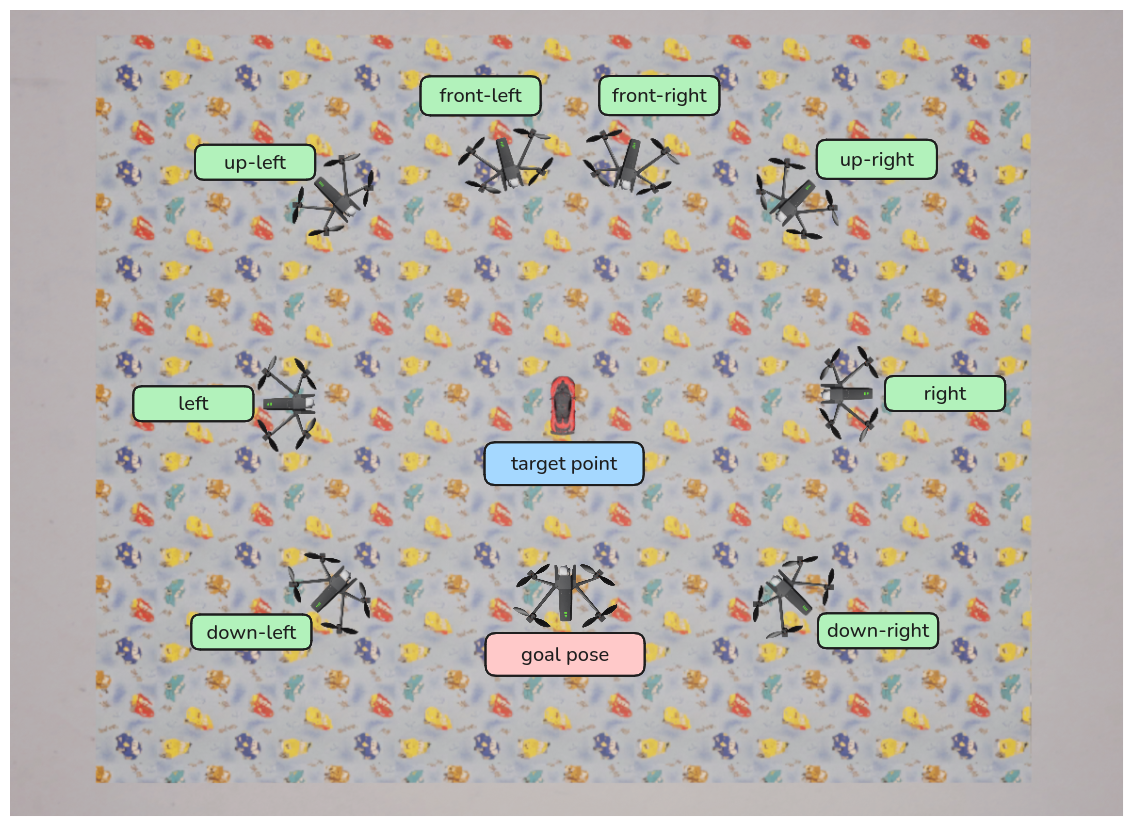
\includegraphics[width=0.8\linewidth]{Drone-Starting-Point.png}
    \caption{原论文中的飞行测试环境配置图，共给出了目标车周围的 8 个起始位姿。无人机必须从每个起始位姿出发，到达车辆正后方的目标位姿，同时保持目标车始终在摄像头视野内。左上、右上、左下和右下四个位姿相对于车辆为 $\pm45^{\circ}$，而左前和右前位姿约为 $\pm14^{\circ}$。}
    \label{fig:drone-starting-poses}
\end{figure}

学生模型仅在上述每个无人机位姿上使用 30 次仿真运行进行训练，共计 240 个训练样本（$74307$ 帧）。训练过程中使用 5 倍数据扩增策略（4 组增强数据 + 1 组原始数据），在每个 epoch 中通过随机饱和度、亮度偏移和椒盐噪声制造合成多样性，同时保留一组原始帧。数据集中的速度命令 $v_x$、$v_y$ 和 $\omega_z$ 按照其分布进行归一化（见表 \ref{tab:cmd-values}），图像则统一缩放到 $224 \times 224$ 像素。由于模型目标是输出速度命令，因此这种缩放不会影响方法性能。训练使用 Adam 优化器，学习率为 0.001，损失函数为均方误差。验证损失采用早停机制监控，耐心值为 3，阈值为 $10^{-4}$。

\begin{figure*}[!ht]
    \centering
    \begin{minipage}[t]{0.48\textwidth}
        \centering
        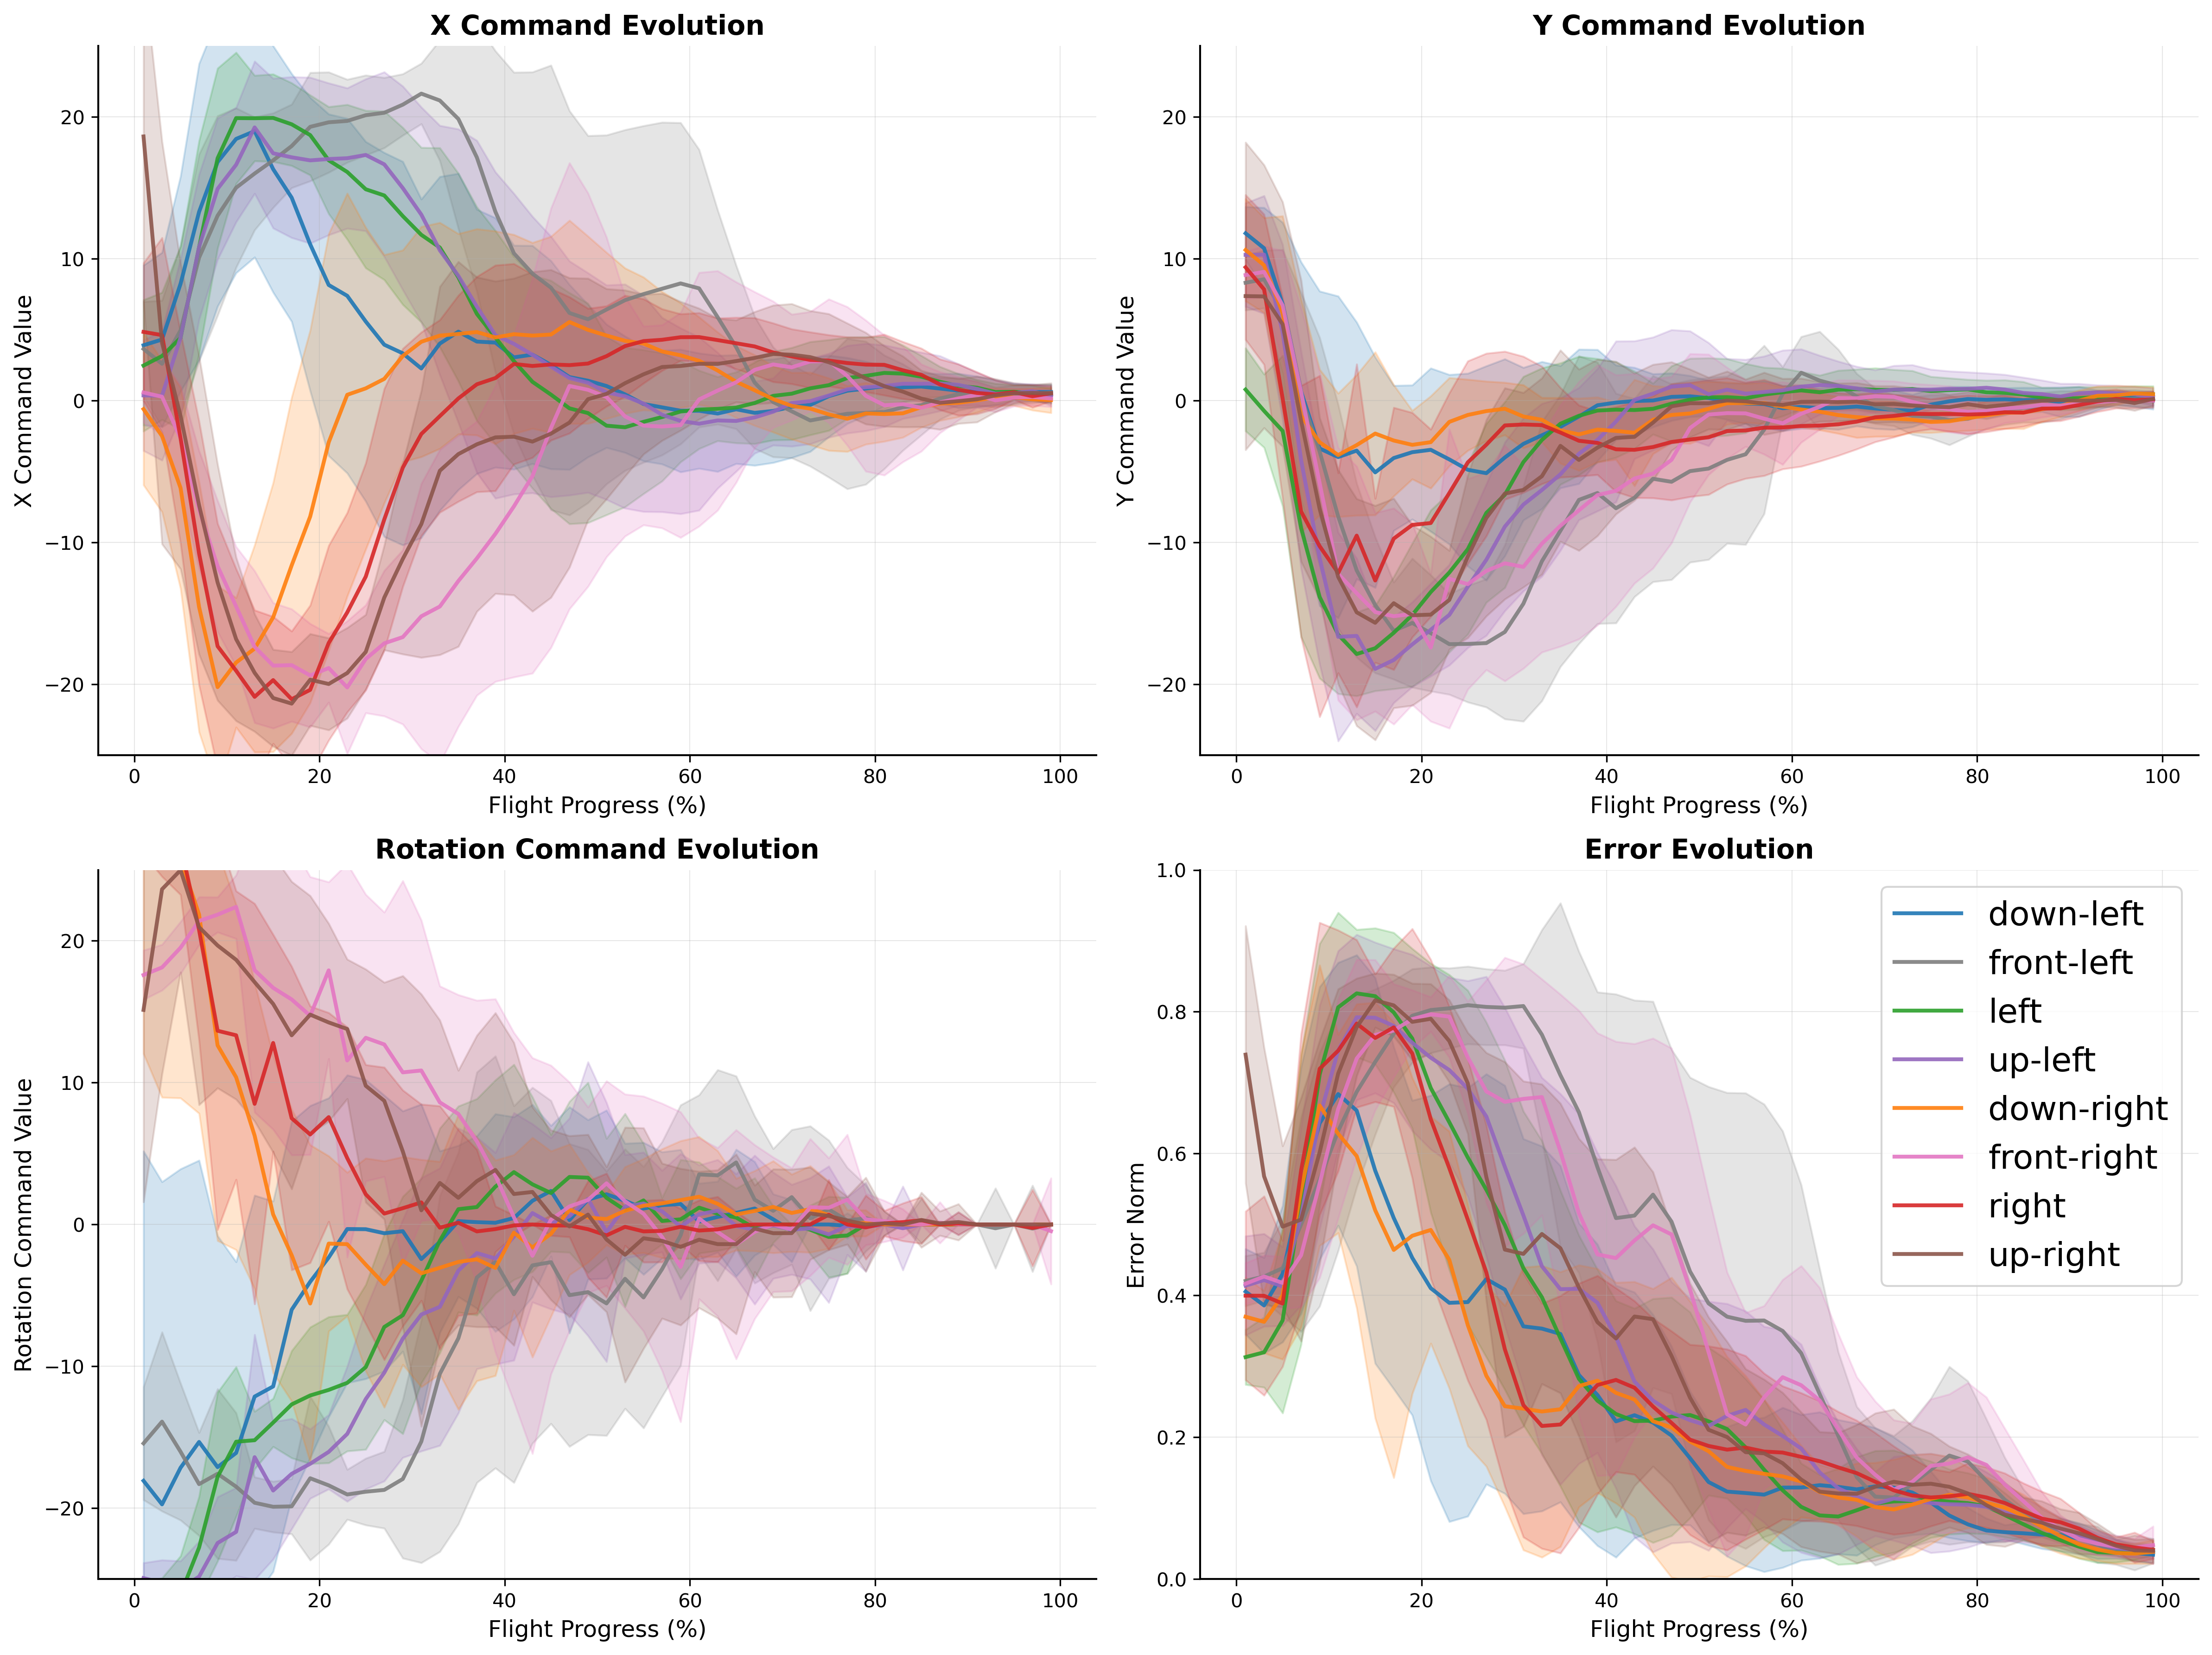
\includegraphics[width=\linewidth]{real_ibvs_evolution_over_time_commands_errors_rl_style_combined.png}
        \caption*{(a) 真实环境中的解析式教师模型（NSER IBVS）：无人机控制命令和跟踪误差随飞行轨迹的变化。}
        \label{fig:real-ibvs-evolution-over-time}
    \end{minipage}
    \hfill
    \begin{minipage}[t]{0.48\textwidth}
        \centering
        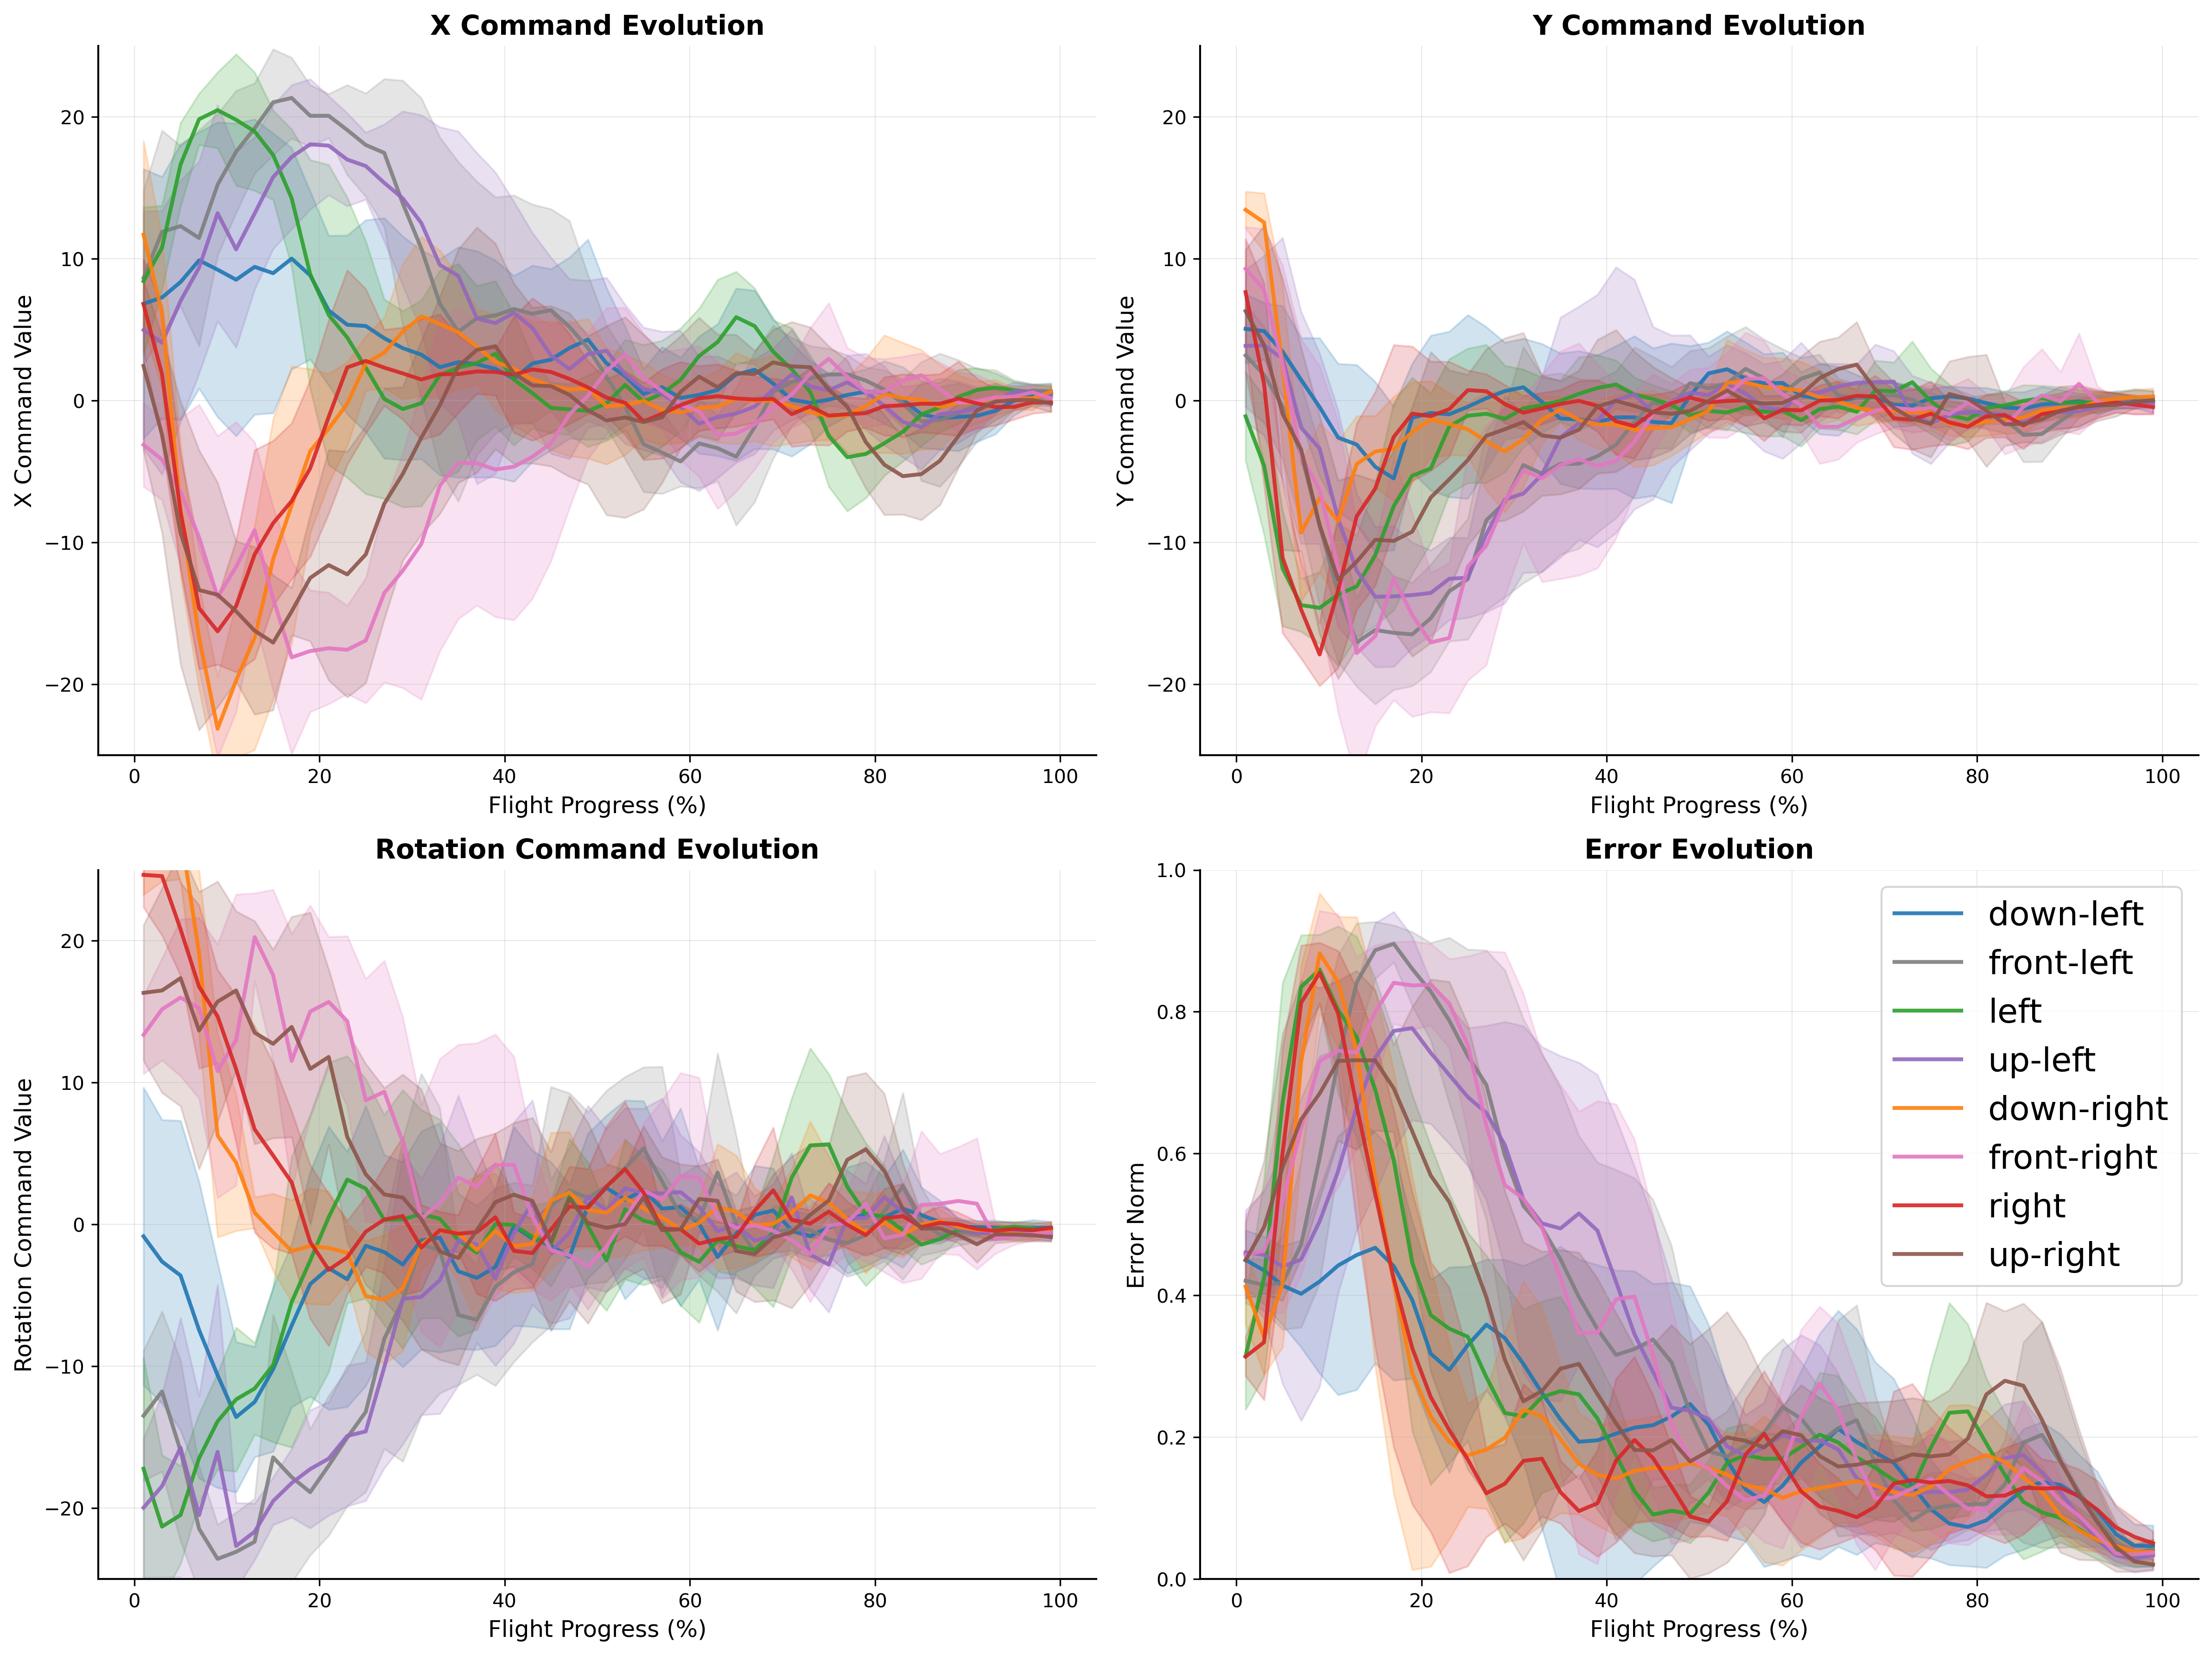
\includegraphics[width=\linewidth]{real_student_evolution_over_time_commands_errors_rl_style_combined.png}
        \caption*{(b) 真实环境中的小型 ConvNet 学生模型：无人机控制命令和跟踪误差随飞行轨迹的变化。}
        \label{fig:real-student-evolution-over-time}
    \end{minipage}
    \caption{在 8 个不同起始位姿上的新测试序列中，教师模型（NSER IBVS）与学生模型（自监督神经解析模型）的无人机控制命令和误差变化对比。实线表示均值，阴影区域表示不同运行之间的波动范围。所有控制命令和误差都收敛到零附近，说明系统能够在各种初始条件下实现稳定的轨迹跟踪和控制收敛。可以看出，复杂的解析式教师模型与小型 ConvNet 学生模型在控制和到目标距离误差上的表现非常相似。}
    \label{fig:real-evolution-comparison}
\end{figure*}

\subsection{任务终止条件}
\label{subsed:experiments-termination-conditions}
我们设计了三种终止条件，所有实验都使用 $640 \times 360$ 像素的图像帧。第一种是 75 秒硬超时，如果无人机在这段时间内未能修正位姿，则自动降落。第二种是软条件：当最近 5 帧误差的中位数 $\leq 80$ 像素，并且连续 3 秒速度命令都保持为 0 时触发，这说明误差已经较小，但可能陷入局部最优。第三种是硬条件：当最近 5 帧误差的中位数连续 3 秒 $\leq 40$ 像素时触发，这表明 NSER IBVS 只生成很小的命令，移动量几乎可以忽略。误差按包含原始像素值向量的 L2 范数计算。

为了在不依赖 IBVS 以及两个神经网络（YOLOv11 和 Mask Splitter）的情况下独立评估学生模型，我们通过分析教师方法的评估统计量，经验性地推导出学生模型的终止条件。我们考察了每次评估运行最后 3 秒内的速度命令值。结果表明，在大多数测试中，速度命令通常落在绝对值 0 到 1 的范围内。因此，我们将其作为仿真中学生模型的终止条件：如果最近 5 个命令的绝对值连续 3 秒都 $\leq 1$，则无人机降落并结束测试。

在真实环境中，测试方法类似，但数据点更少。我们像仿真中一样，针对每个姿态测试了 10 个飞行序列（见图 \ref{fig:drone-starting-poses}），共得到 80 次真实评估，包含 $43963$ 帧。真实部署的学生模型先在 240 次仿真运行上进行预训练，再在真实场景上微调。真实环境中的降落终止条件与仿真一致。

\subsection{评价指标}
\label{subsec:experiments-metrics}
我们使用多个指标比较教师模型和学生模型的性能。主要指标包括最后 3 秒内目标点与当前点之间的 \textbf{误差范数} 和 \textbf{交并比}（IoU）。此外，我们还测量了从跟踪开始（无人机起飞且摄像头向下倾斜 45 度）到降落为止的总 \textbf{飞行时长} 和 \textbf{飞行距离}。对于学生模型，这些指标在离线状态下计算。

\subsection{结果与讨论}
\label{sec:discussions-results}
结果表明，与教师方法相比，学生模型的跟踪精度显著提升。在仿真中，学生模型的平均误差范数为 $14.261$ 像素，而教师模型为 $29.756$ 像素，跟踪精度提升了 $52\%$。IoU 指标也表现出类似的改进，学生模型达到 $0.752$，教师模型为 $0.522$，说明学生模型在目标覆盖和定位方面更好 \ref{tab:teacher-student-metricwise}。

\begin{table*}[htpb]
    \centering
    \small
    \setlength{\tabcolsep}{4pt}
    \renewcommand{\arraystretch}{0.9}
    \begin{tabular}{c c c c c c c c}
         &  & \multicolumn{1}{c}{\makecell{仿真飞行 \\ (距离(m) / 时间(s)) $\downarrow$}} & \multicolumn{1}{c}{\makecell{仿真 \\ 误差范数 (px) $\downarrow$}} & \multicolumn{1}{c}{仿真 IoU $\uparrow$} & \multicolumn{1}{c}{\makecell{真实飞行 \\ (距离(m) / 时间(s)) $\downarrow$}} & \multicolumn{1}{c}{\makecell{真实误差范数 (px) $\downarrow$}} & \multicolumn{1}{c}{IoU $\uparrow$} \\
        \addlinespace
        \cmidrule(lr){3-5} \cmidrule(lr){6-8} \multirow{2}{*}{左上} & 教师 & 5.312 / \textbf{23.466} & 29.256 & 0.530 & 5.798 / \textbf{36.721} & 30.134 & 0.620 \\
                               & 学生 & \textbf{5.193} / 24.164 & \textbf{13.319} & \textbf{0.759} & \textbf{5.735} / 43.334 & \textbf{28.600} & \textbf{0.6263} \\
        \addlinespace
        \multirow{2}{*}{右上} & 教师 & \textbf{5.675 / 24.226} & 31.800 & 0.503 & \textbf{5.622 / 41.581} & 31.499 & 0.621\\
                               & 学生 & 6.064 / 28.298 & \textbf{13.172} & \textbf{0.766} & 5.716 / 45.885 & \textbf{22.802} & \textbf{0.6919}\\
        \addlinespace
        \multirow{2}{*}{左前} & 教师 & 6.196 / \textbf{27.315} & 30.706 & 0.517 & 6.493 / \textbf{37.535} & \textbf{28.54} & \textbf{0.611}\\
                               & 学生 & \textbf{6.041} / 27.917 & \textbf{13.430} & \textbf{0.758} & \textbf{6.490} / 47.238 & 33.981 & 0.560\\
        \addlinespace
        \multirow{2}{*}{右前} & 教师 & \textbf{6.846 / 32.358} & 32.608 & 0.488 & \textbf{6.197 / 37.166} & 33.15 & \textbf{0.658}\\
                               & 学生 & 7.043 / 35.535 & \textbf{18.028} & \textbf{0.718} & 6.316 / 46.363 & \textbf{31.035} & 0.627\\
        \addlinespace
        \multirow{2}{*}{左} & 教师 & 4.177 / \textbf{20.228} & 31.453 & 0.519 & \textbf{4.559 / 29.921} & \textbf{28.015} & 0.629\\
                               & 学生 & \textbf{4.089} / 20.481 & \textbf{13.243} & \textbf{0.762} & 5.065 / 43.841 & 30.853 & \textbf{0.6482} \\
        \addlinespace
        \multirow{2}{*}{右} & 教师 & \textbf{4.317 / 19.637} & 31.137 & 0.494 & 4.831 / \textbf{41.409} & \textbf{32.423} & \textbf{0.612}\\
                               & 学生 & 4.518 / 21.987 & \textbf{13.798} & \textbf{0.759} & \textbf{4.811} / 57.245 & 43.672 & 0.5 \\
        \addlinespace
        \multirow{2}{*}{左下} & 教师 & 2.779 / 15.988 & 28.473 & 0.518 & 4.384 / \textbf{31.622} & \textbf{28.00} & \textbf{0.611}\\
                               & 学生 & \textbf{2.777 / 14.900} & \textbf{13.257} & \textbf{0.763} & \textbf{4.326} / 41.044 & 39.531 & 0.5253 \\
        \addlinespace
        \multirow{2}{*}{右下} & 教师 & \textbf{2.893 / 13.667} & 22.618 & 0.606 & 4.137 / \textbf{33.523} & \textbf{27.89} & \textbf{0.654}\\
                               & 学生 & 3.145 / 17.035 & \textbf{15.839} & \textbf{0.728} & \textbf{3.938} / 38.001 & 36.195 & 0.5478 \\
        \bottomrule
        \addlinespace
        \multirow{2}{*}{平均} & 教师 & \textbf{4.774 / 22.111} & 29.756 & 0.522 & \textbf{5.253 / 36.185} & \textbf{29.956} & \textbf{0.627}\\
                               & 学生 & 4.859 / 23.790 & \textbf{14.261} & \textbf{0.752} & 5.300 / 45.369 & 33.334 & 0.591 \\
        \bottomrule
    \end{tabular}
    \caption{不同起始位姿下的教师-学生比较。左侧为仿真结果，右侧为真实飞行结果。指标包括总飞行距离/时间、最终像素误差范数（对 4 个角点组成的误差向量求 L2 范数）以及最终 IoU（均在飞行最后 3 秒内计算）。教师在飞行时间上略快，但学生在计算时间上快 $11\times$（见表 \ref{tab:nn-timing-eval}）。学生在仿真中略更准确，因为训练更充分；但在真实环境中，由于真实飞行次数较少，其精度略低于教师。}
    \label{tab:teacher-student-metricwise}
\end{table*}

轨迹演化分析表明，两种方法都能成功收敛到目标，但表现特征不同。教师方法的控制命令更保守，收敛更平缓；学生方法则采用更直接的路径，误差下降速度更快，如图 \ref{fig:trajectory-ibvs} 所示。

\begin{figure}
    \centering
    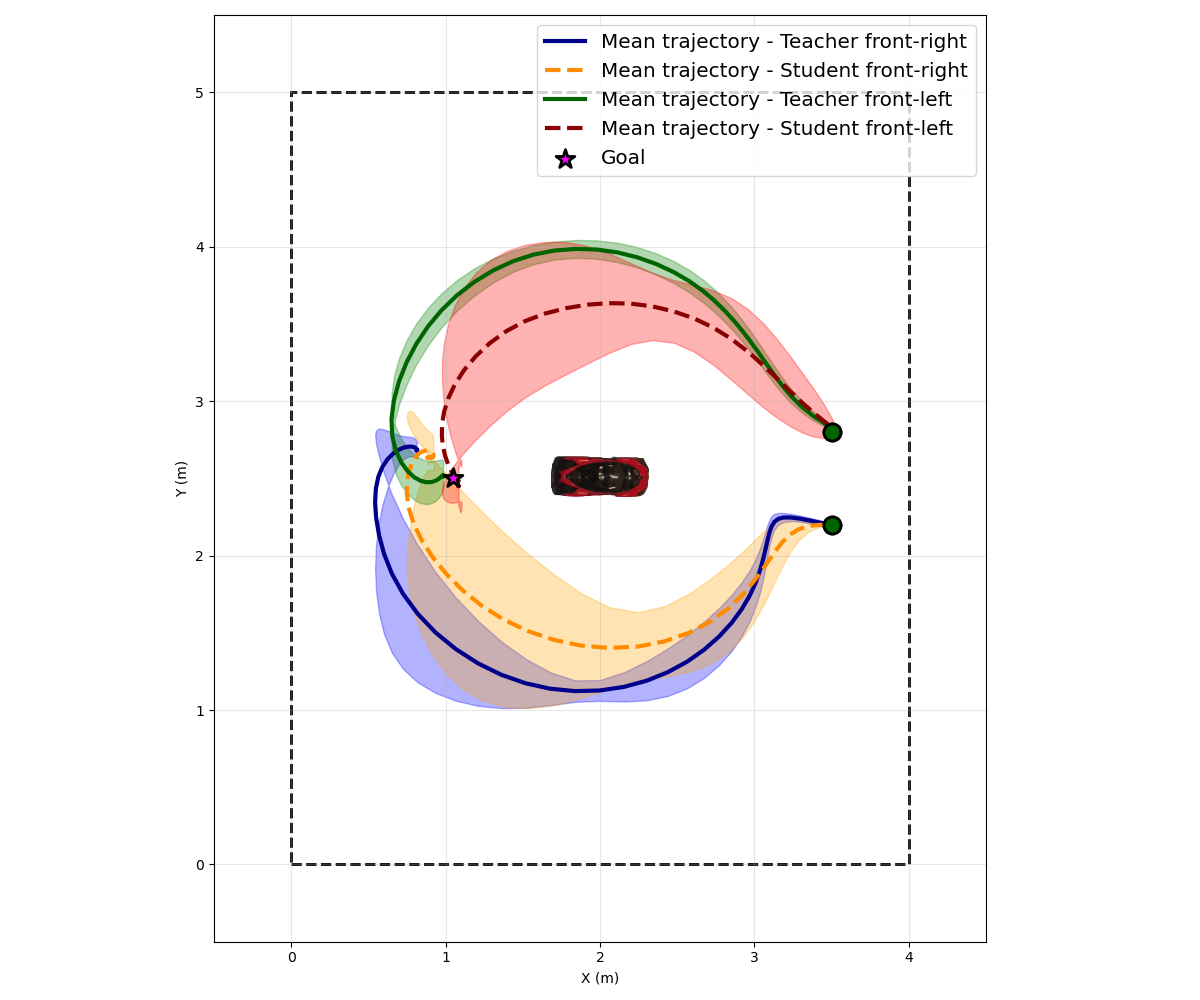
\includegraphics[width=\linewidth]{trajectories_sim_teacher_student_front.png}
    \caption{教师和学生在仿真飞行中的轨迹对比，给出了两个起始位姿（绿色圆点：左前和右前）的均值与标准差。蓝色和绿色实线表示教师 NSER IBVS 方法的平均路径，橙色和红色虚线表示学生路径。阴影区域表示不同运行之间的轨迹波动。星号表示目标位姿。可以看到，学生路径波动更大，但其平均路径长度短于教师。}
    \label{fig:trajectory-ibvs}
\end{figure}

为了比较本文提出的学生网络在有无分割情况下与基线 NSER IBVS 之间的计算效率，我们在一组分辨率为 $640 \times 360$ 的真实世界帧上进行了运行时间基准测试。每个评估器都独立处理同一组输入帧，并对每帧的推理时间重复测量 30 次，以考虑系统负载和内存效应带来的波动。每次试验前都进行了预热迭代以避免初始化偏差，并在试验间显式释放内存。我们以毫秒和 FPS 表示推理时间。结果汇总于表 \ref{tab:nn-timing-eval}。

\begin{table}[t]
\centering
\footnotesize
\caption{30 次试验的计算时间（毫秒）。小型 1.7M 参数学生 ConvNet 比教师快 $11\times$。}
\label{tab:nn-timing-eval}
\begin{tabular}{lrrrrrr}
\toprule
\textbf{评估器} & \textbf{平均} & \textbf{标准差} & \textbf{中位数} & \textbf{最小值} & \textbf{最大值} & \textbf{FPS} \\
\midrule
NSER IBVS & 20.69 & 7.63 & 24.56 & 6.45 & 82.55 & 48.30 \\
学生 & \textbf{1.85} & 0.93 & 1.84 & 1.79 & 235.64 & \textbf{540.8} \\
\bottomrule
\end{tabular}
\end{table}

结果表明，该方法实现了有效的仿真到现实迁移，但正如预期那样存在一定性能下降。在真实世界场景中，学生模型保持了具有竞争力的跟踪精度，而教师模型在不同环境中表现更稳定。使用 80 个真实场景进行微调的做法验证了领域自适应的有效性，并有助于在实际场景中成功部署。

\section{总结与结论}
\label{sec:conclusion}
本文提出了首个用于无人机视觉伺服的自监督神经解析系统，并通过高效知识蒸馏实现：一个小型 ConvNet 学生从所提出的、数值稳定的解析式教师（NSER-IBVS）中学习，使无人机能够从不同起始位姿飞到目标位姿，而这些起始位姿在三角函数圆上充分覆盖了相对位姿差异。该系统完全不需要人工干预、监督预训练或外部传感器，与文献中的其他方法不同。该学生网络只有 1.7M 参数，易于部署在嵌入式设备上，其计算速度比教师路径快 $11\times$（$529.77$ FPS 对比 $48.3$ FPS），同时在仿真和真实世界测试中都保持了相近的准确率和飞行速度。真实场景学习仅依赖 80 次飞行，从而通过数字孪生仿真环境与真实场景之间的高效迁移进一步降低了成本。

本文提出的两阶段分割管线结合 YOLOv11 与专门的基于 U-Net 的掩码分裂器，无需显式几何模型或 fiducial marker，即可提供稳健的车辆前后区域分割。该方法的自监督特性已经通过仿真到现实迁移学习得到验证，并在 Parrot Anafi 无人机平台上进行了测试，表明其在最小硬件基础设施条件下实现完全自主室内操作具有现实可行性。

跨不同无人机位姿、并完整覆盖三角函数圆的实验验证，进一步确认了该无监督方法的有效性。虽然学生网络在真实环境中的像素误差略高于教师模型（平均误差分别为 $29.956$ 和 $33.334$ 像素），但其 IoU 性能仍可接受（$0.627$ 与 $0.591$），并且收敛更快。尤其是在仿真环境中，随着更充分的自监督训练进行，系统表现出更优的收敛速度和更低的误差，这验证了与昂贵的真实数据采集相比，基于仿真的训练方式更具成本效益。计算效率的提升使得该方法在资源受限平台上的实时应用尤其有价值，并为无需人工监督或标记依赖的自主视觉伺服建立了新的范式。

\section*{致谢}
本文部分受以下项目资助："Romanian Hub for Artificial Intelligence - HRIA"，Smart Growth、Digitization and Financial Instruments Program, 2021-2027（MySMIS 编号 334906）；European Health and Digital Executive Agency（HADEA）在欧盟委员会授权下资助的 DIGITWIN4CIUE 项目（资助协议编号 101084054）；以及 "European Lighthouse of AI for Sustainability - ELIAS"，Horizon Europe 计划（资助编号 101120237）。
{
\small
\bibliographystyle{ieeenat_fullname}
\bibliography{main}
}

\end{document}
\typeout{get arXiv to do 4 passes: Label(s) may have changed. Rerun}
